% Package
\documentclass[11pt]{article}

\usepackage{amsmath}
\usepackage{cite}
\usepackage{graphicx}
\usepackage[utf8]{inputenc}
\usepackage[T1]{fontenc}
\usepackage{lmodern}

\title{ADP Aufgabe 1, Abgabe 1}
\author{Team 1\\Hugo Protsch, Justin Hoffmann}

% Document
\begin{document}

    \maketitle


    \section{Formales}\label{sec:Formales}

    %! suppress = MissingLabel

    \subsection{Aufgabenaufteilung}
    Der Code wurde zusammen entwickelt.
    %! suppress = MissingLabel

    \subsection{Quellenangaben}
    
    Es wurden lediglich Vorlesungsmaterialien verwendet.

    %! suppress = MissingLabel

    \subsection{Bearbeitungszeitraum}
    Für die Bearbeitung des Entwurfs haben wir in etwa 8 bis 10 Stunden
    benötigt.
    Für die Entwicklung des Quellcodes haben wir in etwa 10 bis 15 Stunden
    benötigt.
    %! suppress = MissingLabel

    \subsection{Aktueller Stand}
    Der Quellcode ist funktionsfähig und wurde auf Laufzeit überprüft.

    %! suppress = MissingLabel

    \subsection{Änderungen des Entwurfes}
    -- nicht zutreffend --


    \section{Laufzeitmessung}\label{sec:laufzeitmessung}
    \subsection{Zufällig}\label{subsec:zufaellig}



    \begin{center}
        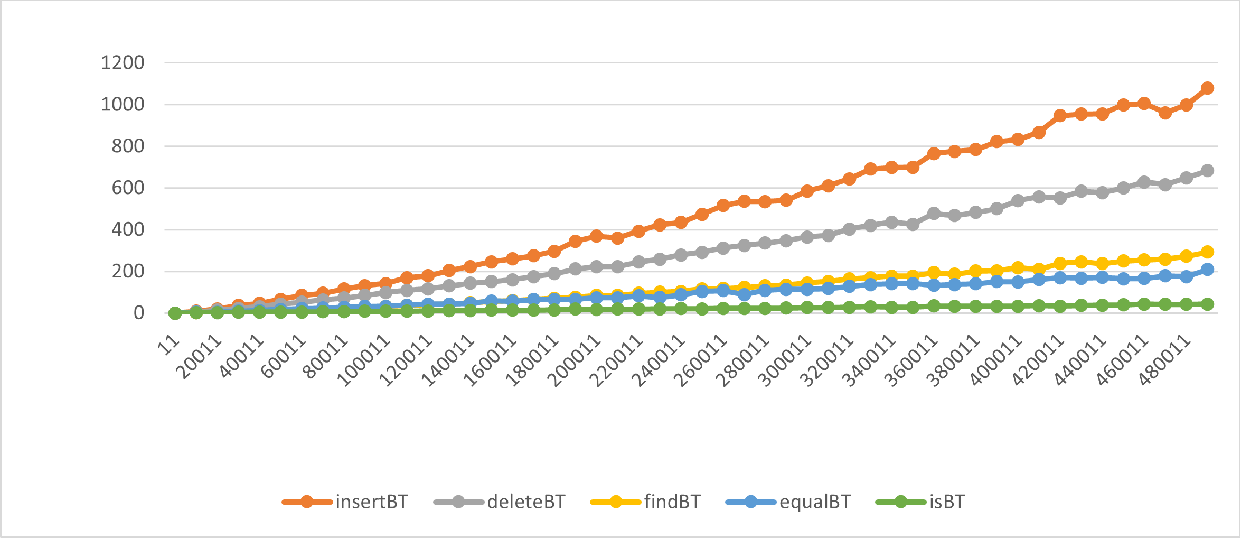
\includegraphics[width=0.9\columnwidth] {ZeitAvg.pdf}
    \end{center}

    \subsection{Aufsteigend und Absteigend}\label{subsec:average}
    \begin{center}
        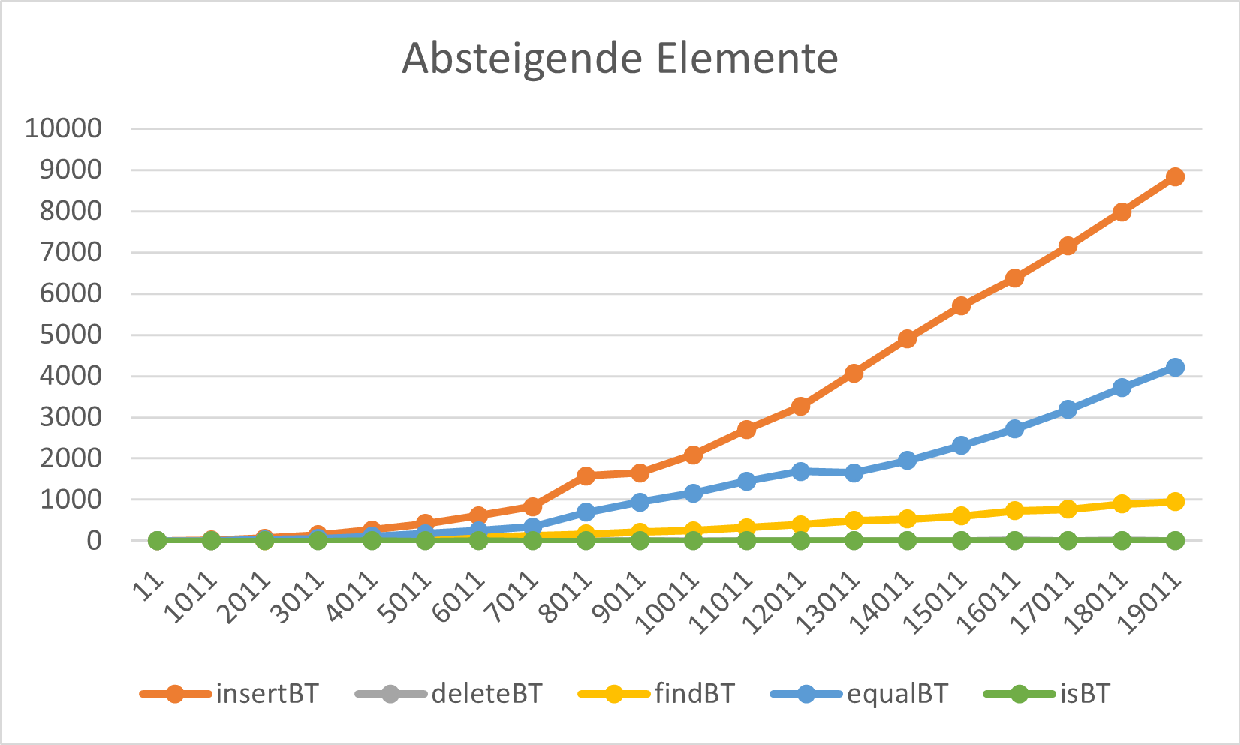
\includegraphics[width=0.9\columnwidth] {ZeitAb.pdf}

    \end{center}\begin{center}
                    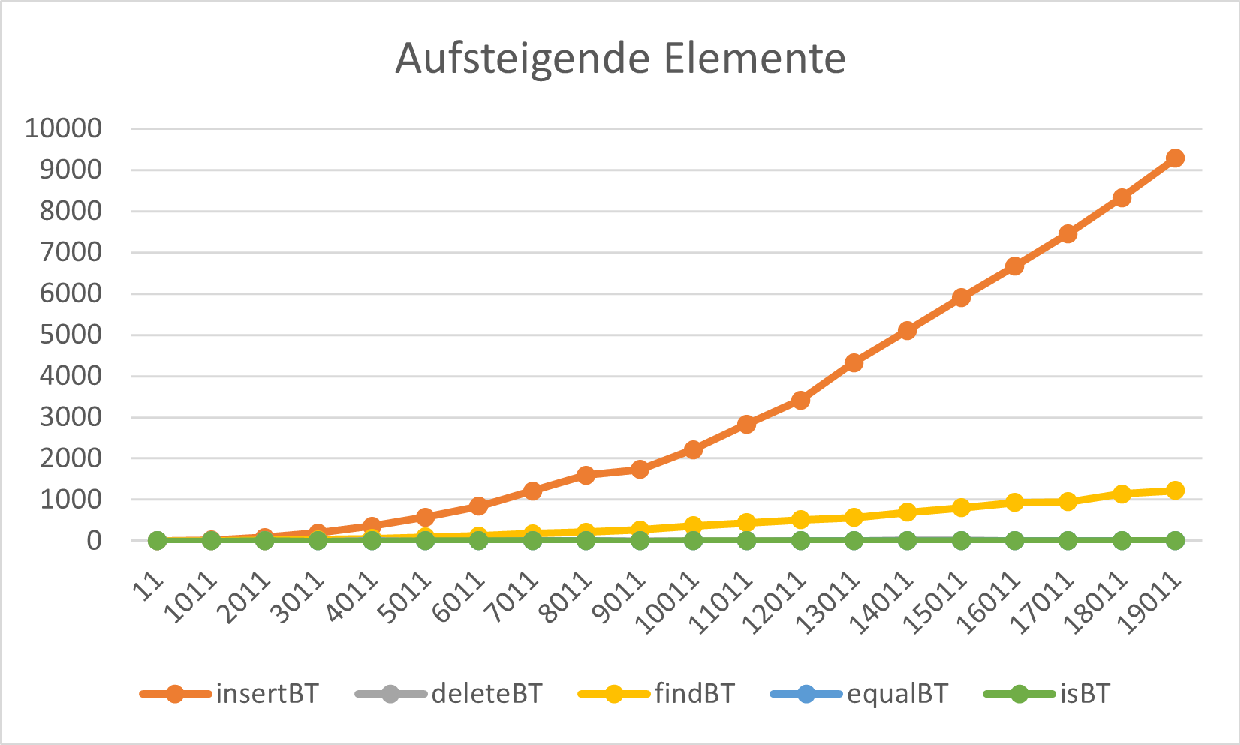
\includegraphics[width=0.9\columnwidth] {ZeitAuf.pdf}
    \end{center}

    Für den Versuch der Laufzeitmessung werden jeweils die Funktionen mit
    variierender Elementanzahl getestet. Beginnend bei
    annähernd 0 Elementen wird die Anzahl jeweils um eine feste Schrittgröße
    erhöht. Hierbei ist das Ziel, die Schrittgröße so zu wählen, dass bei 20
    Schritten eine maximale Laufzeit von ca. 5 Sekunden (5000ms) erreicht
    wird. Wir mitteln über 3 Durchgänge.
    Falls die Abweichungen zwischen den Durchgängen zu groß sind, kann die
    Anzahl der dieser nachträglich angepasst werden.

    Es werden drei Messungen, eine mit zufälligen, eine mit
    aufsteigenden und eine mit absteigenden Zahlen, ausgeführt.
    Bei absteigenden und aufsteigenden Zahlen erwarten wir jeweils den
    Worst-Case, bei zufälligen den Average-Case.

    Die Laufzeit wird anschließend mit besagter Eingangsgröße in Relation gesetzt.
    Wir vergleichen den gemessenen funktionellen Zusammenhang mit dem Erwarteten,
    welcher in den Entwürfen der jeweiligen Funktion beschrieben ist.

    Die Rahmenbedingungen der Messung sind hierbei vorgegeben.

\end{document}
